\documentclass[11pt]{beamer}

\usepackage[utf8]{inputenc}
\usepackage[magyar]{babel}
\usepackage[T1]{fontenc}
\usepackage{lmodern}
\usepackage{zi4}
\usepackage{multirow}
\usepackage{listings}
\usepackage{ragged2e} % For \justifying command

\usetheme{Warsaw}

\renewcommand\UrlFont{\ttfamily\footnotesize}

% no navigation symbols
\setbeamertemplate{navigation symbols}{} 

% frame numbers
\expandafter\def\expandafter\insertshorttitle\expandafter{%
  \insertshorttitle\hfill%
  \insertframenumber\,/\,\inserttotalframenumber}

\author{Gregorics Tibor, Nagy András}
\title{Tapasztalatok az osztály-sablon könyvtár bevezetésével}
\date{2018. november 24.}

\logo{%
	\makebox[0.95\paperwidth]{%
		\hfill%
		
\includegraphics[width=3.2cm,keepaspectratio]{efop-logo.jpg}%
	}%
}

\begin{document}

\begin{frame}
\titlepage
\end{frame}

\begin{frame}
	\frametitle{Osztálysablon könyvtár bemutatása}
	
	\begin{itemize}
		\item Nevezetes programozási tételeket leíró osztályokat tartalmaz
		\item Konkrét feladatok megoldása esetén leszármazással dolgozunk, visszavezetve a problémát egy nevezetes tételre
		\item Az adott feladatra jellemző tulajdonságokat és értékeket adhatjuk meg. (Pl. számlálásnál a feltételt)
		\item A feldolgozandó elemek felsorolóját futás időben adjuk meg (Függőség befecskendezés)
	\end{itemize}
\end{frame}

\begin{frame}[fragile]
	\frametitle{Osztálysablon könyvtár bemutatása}
	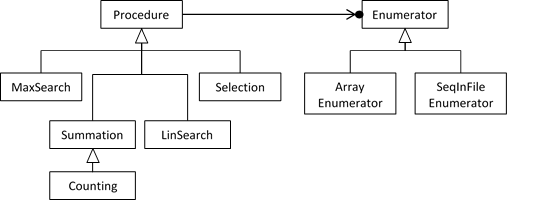
\includegraphics[scale=0.8]{sablon_hiearhica.png}
	
	\begin{block}{run() metódus}
		\begin{lstlisting}[basicstyle=\small]
init();
for (enor->first(); !enor->end(); enor->next()) {
    body(enor->current());
}
		\end{lstlisting}
	\end{block}
	
\end{frame}


\begin{frame}[fragile]
	\frametitle{Osztálysablon könyvtár bemutatása - Példa}	
	\begin{block}{Feladat}
		Számítsuk ki egy C++ vektorban elhelyezett számok összegét.
	\end{block}
	
	Az alábbiakat kell meghatározni a megoldásához:
	\begin{itemize}
		\item Összegzéssel oldjuk meg a feladatot
		\item A feldolgozandó elemek, valamint az eredmény típusa is ugyanaz (egész szám).
		\item Az összegző művelet egyszerű összeadás, a neutrális elem a 0.
		\item Egy \textit{std::vector} elemeit kell felsorolni.
	\end{itemize}

	
\end{frame}

\begin{frame}[fragile]	
	\begin{block}{Megoldó osztály}
		\begin{lstlisting}[basicstyle=\small]
class SimpleSum : public Summation<int,int> {
public:
 int add(const int& a, const int& b) const {
  return a + b;
 }
 int neutral() const {return 0;}
 int func(const int& e) {return e;}
}
		\end{lstlisting}
	\end{block}
	
	\begin{block}{Osztály használata}
	  	\begin{lstlisting}[basicstyle=\small]
SimpleSum sum;
ArrayEnumerator e({1,2,3});
sum.addProcedure(&e);
sum.run();
		\end{lstlisting}
	\end{block}
\end{frame}

\begin{frame}
	\frametitle{Az osztálysablon könyvtár bevezetése az oktatásba}
	\begin{itemize}
		\item 2009-ben vezettük be az oktatásba
		\vspace*{2px}
		\item A célja az újrafelhasználás gyakorlása volt
		\vspace*{2px}
		\item Számos negatív és pozitív tapasztalat gyűlt össze
		\vspace*{2px}
		\item Ezeket tapasztalatokat felhasználva megreformáltuk a könyvtárat
	\end{itemize}
\end{frame}

\begin{frame}
	\frametitle{Pozitívumok}
	\begin{itemize}
		\item Robusztus könyvtár, sok feladat megoldására alkalmas
		\item Objektumorientált technológiák bemutatása, gyakorlása (leszármazás, függőség befecskendezés, stb..) 
		\vspace*{8px}
		\item Visszavezetéses technikák gyakorlása
		\vspace*{8px}
		\item Rákényszeríti a hallgatót az elemzésre, tervezésre egyszerű feladatok esetén is
		\item C++ objektumorientált nyelvi elemek mélyítése, gyakorlása (sablonok, metódusok felül definiálása, stb..)
		
	\end{itemize}
\end{frame}

\begin{frame}
	\frametitle{Problémák, kritikák}
	\begin{itemize}
		\item Kritikák
		\begin{itemize}
			\item Iparban nem használt könyvtár
			\item Nagyobb kódméret, túl erős technológiákra épül
			\item Elavult C++ nyelvi konvenciók
		\end{itemize}
		\item Problémák
		\begin{itemize}
			\item Nem szakszerűen használták: Egyre bővülő szabályrendszert kellett  bevezetni, hogy helyesen használják a hallgatók (mit lehet felüldefiniálni, kiből lehet származni..)
			\item Összegzés tétele túl általános volt
		\end{itemize}
	\end{itemize}
\end{frame}

\begin{frame}[fragile]
	\frametitle{Összegzés módosításai}
	\begin{block}{Új összegzés metódusai}
	\begin{lstlisting}[basicstyle=\small]
void  init() override final{_result=neutral();}
void  body(const Item& e) override final {
 if(cond(e))_result = add(_result,e);
}
void  cond(const Item& e){return true;}
Value add(const Item& a, const Item& b) const = 0;
Value neutral() const = 0;
Value func(const Item& e) const = 0;

	\end{lstlisting}
	\end{block}
	
	\begin{itemize}
	\item Neutrális elem, összeadás művelet, leképező művelet bevezetése
	\item Az \textit{add} nem volt konstans, nagyon általános volt, ő változtatta meg az eredmény értékét tetszőleges módon
	\end{itemize}
\end{frame}

\begin{frame}
	\frametitle{Új felsorolók}
		 \textit{StringStreamEnumerator} 
		 \begin{itemize}
		 	\item Változó hosszúságú sor beolvasásakor hasznos.
		 	\item C++ specifikus
		 	\item Példa: Egy sor egy receptet tartalmaz (pl: "tej 1 liter búzadara 13 evőkanál vaj 6 dkg cukor 5 evőkanál") A recept összetevőit szeretnék eltárolni egy tömbben.
		 	\item Összegzéssel megoldva: Az \textit{add} művelet az összefűzés, a semleges elem az üres tömb.
		 \end{itemize}
		
		\textit{IntervalEnumerator}
		\begin{itemize}
			\item Egy $[m,n]$ diszkrét intervallum értékeit sorolja fel
			\item Példa: Egy n szám faktoriálisa összegzéssel. Ilyenkor az intervallum $[2,n]$, az \textit{add} művelet egy összeszorzás, a semleges elem pedig az 1.
		\end{itemize}
		
\end{frame}

\begin{frame}
	\frametitle{Új nyelvi elemek}
	\begin{itemize}
		\item Final: Nem engedi a leszármazott osztályokban felül definiálni az adott metódust. (pl. az összegzésben a body-t) Nem kell külön kikötni, mit nem definiálhatnak felül a használata során.
		\item Override: Jelzi, hogy felül definiáljuk egy ősosztály metódusát. Csökkenti a hibázási lehetőségeket a zárthelyiken, ha a hallgatók is használják.
		\item Barát osztályok bevezetése: Korlátozzuk, hogy a \textit{Procedure} ősosztályból csak a tételek osztályai származhatnak le. (Nem kell külön kikötni, hogy nem származhatnak le az ősosztályból.)
		\item Template specializáció: Fájl létrehozó metódus specializálása karakterekre. Javít a kód konvencióján, az új összegzésnél elengedhetetlen összefűzések esetén.
		\item \textit{nullptr}, \textit{pagrma once}..
	\end{itemize}
\end{frame}

\begin{frame}
	\frametitle{Összefoglalás, eredmények}
	\begin{itemize}
		\item Új helyre került a könyvtár bevezetése, a felsorolós programozási tételek után tanulják közvetlenül, gyakorolva a visszavezetési technikákat.
		\item Javult a könyvtár kódjának tisztasága.
		\item Az új nyelvi elemekkel elősegítettük a szakszerű használatot, nincs szükség annyira kikötésre.
		\item A könyvtár hasznos didaktikai eszköznek bizonyult. (Hangsúlyozni kell a hallgatóknak a könyvtár célját..)
	\end{itemize}
\end{frame}

\begin{frame}
	\frametitle{Tapasztalatok az osztály-sablon könyvtár bevezetésével}
	\begin{center}
		\Large{Köszönöm a figyelmet!}
	
	\vspace*{25px}
	{\small A projekt az Európai Unió támogatásával, az Európai Szociális Alap társfinanszírozásával valósult meg (EFOP-3.6.3-VEKOP-16-2017-00002).}\end{center}
\end{frame}

\end{document}
